\documentclass[../main]{subfiles}
\ifSubfilesClassLoaded{
    \dominitoc
    \tableofcontentsfile
	\pagenumbering{arabic}
    \setcounter{page}{1}
}{}
\begin{document}
\chapter{Analyse de l'auto-organisation de CxSOM sur des cartes en une dimension}\label{chap:analyse}
\graphicspath{{06-Analyse/figures},{./figures}}
\minitoc

Nous avons proposé un modèle de connexions de cartes auto-organisatrices au sein d'une architecture complète s'appuyant sur un consensus~; le but de ce chapitre est de définir et comprendre des mécanismes d'auto-organisation occurrant dans des cartes en une dimension et permettant d'apprendre une relation entre entrées multimodales.
Nous chercherons par la suite à généraliser le comportement aux cartes en deux dimensions.

\`{A} partir des comportements que nous observerons sur plusieurs ensembles de données, 
\`{A} l'issue de ce chapitre, nous serons donc en mesure de construire des architectures de 2 et 3 cartes et d'identifier leur capacité d'apprentissage. 
Nous conclurons sur la scalabilité du modèle à des architectures comportant un plus grand nombre de cartes.

\section{Méthode expérimentale}

Nous utiliserons en premier lieu des modèles géométriques d'entrées. Ces modèles nous permettent de maîtriser les dépendances sur des modalités en basse dimension et ainsi de visualiser les liens entre organisation et apprentissage. Cela nous permettra également de mesurer l'apprentissage de cette dépendance connue au sein des structures de cartes.

\subsection{Entrées}

La dépendance entre modalités est définie par la dimension choisie pour $U$.
Une variable $U$ en une dimension paramètre des points placés sur une courbe en une dimension~; $U$ en 2 dimensions paramètre une surface 2D. 
Plus généralement, quelle que soit la dimension totale $n$ des entrées, nous prendrons ces entrées placées sur une variété de dimension inférieure, $k$,  définie par $U \in [0,1]^k$ et qui définit la dépendance entre entrées. 
Ce modèle est général~: au pire, $U$ correspond à la dimension totale des entrées. Par ailleurs, de nombreux modèles d'entrées réelles se placent sur une variété (\emph{manifold}) de dimension réduite, comme nous l'avions vu au chapitre \ref{chap:repr} pour des images d'un même objet 3D vu par différents angles. 
% La qualité de la décomposition de MNIST par des algorithmes de réduction de dimension tels que t-sne ou même une SOM suggère également que les images se placent sur un manifold de dimension plus f
% L'hypothèse que la majorité des entrées réelles se placent sur une variété de dimension plus faible ( \emph{Manifold hypothesis}) est une hypothèse en apprentissage automatique qui a été 
% \cite{fefferman_testing_2016}
% Bien que cette h
Le choix d'un modèle d'entrées géométriques situées sur une variété de dimension inférieure est donc justifié comme modèle expérimental simplifié.

Nous considérons d'abord des points liés par $U$ en une dimension, situés sur une courbe. 
La dépendance entre entrées varie ensuite en fonction de cette courbe pour une même dimension de $U$. Nous choisissons dans cette section de s'intéresser à différentes dispositions d'entrées qui nous apparaissent pertinentes.

Nous réutiliserons d'abord l'expérience présentée au chapitre représentation, sur des données disposée en cercle. L'intérêt de cette courbe est que la disposition est symétrique~: toute entrée $X^{(1)}$ correspond à deux valeurs possible pour $X^{(2)}$ et inversement.
Nous ferons varier cette propriété de dépendance en observant également le comportement de deux cartes sur des entrées identiques (cas dégénéré). Ces points sont toujours sur une courbe 1D, mais leur dépendance est bijective.
Au contraire, nous étudierons le comportement des cartes sur des entrées totalement indépendantes, prises aléatoirement dans un carré $[0,1]^n$.
Entre ces deux cas dégénérés, nous observerons le comportement d'une architecture sur des exemples implémentant des dépendances variées, par exemple si $X\m{2}$ est une fonction de $X\m{1}$.
Enfin, une carte de Kohonen classique a comme propriété d'être résistante au bruit des données. Ainsi, une carte 1D se dépliant sur un anneau fin en 2D apprendra d'abord la représentation du cercle. Nous voulons vérifier comment cette propriété se vérifie sur l'apprentissage de données par trois cartes~; nous prendrons ainsi des points sur un anneau fin.
Nous lancerons l'apprentissage de structures de deux cartes connectées réciproquement sur ces différents jeux d'entrées, comme proposé au chapitre \ref{chap:repr} et tracerons les représentations. 
Dans un premier temps, nous étudions des architectures de deux cartes 1D, ce qui nous permettra de mieux comprendre certains mécanismes d'organisation.
Nous étendons ensuite notre étude à des architectures de 3 cartes en une dimension, toutes connectées. Nous appliquerons ces architectures à une courbe ($U$ 1D) mais sur trois dimensions, chacune des cartes prenant une des dimensions d'un point comme entrée \ref{fig:cercle3}. Il s'agit ici d'un cercle en deux dimensions que nous pivotons sur la troisième dimension. De cette manière, il existe une redondance entre $X\m{1}, X\m{2}$ et $X\m{3}$ : étant donné $X\m{1}, X\m{2}$ et le modèle d'entrée, il est possible d'en déduire l'entrée manquante.

Dans ce cadre, nous réaliserons de la prédiction d'entrée par les cartes. Nous donnons en entrées $X\m{1}, X\m{2}$ à la structure et verrons si la valeur de $X\m{3}$ correspondante est correctement prédite. Une bonne prédiction témoignera de l'apprentissage du modèle d'entrées par l'architecture de cartes.


\begin{figure}
	\begin{minipage}{\textwidth}
		\begin{minipage}{0.33\textwidth}
			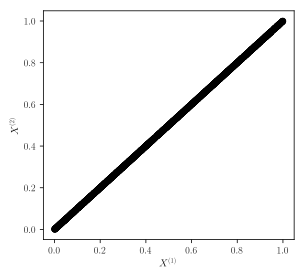
\includegraphics[width=\textwidth]{2som_id_in.pdf}
			\caption{Cas dégénéré d'entrées en deux dimensions~: $X\m{1}$ = $X\m{2}$ \label{fig:id}}
		\end{minipage}
		\begin{minipage}{0.33\textwidth}
			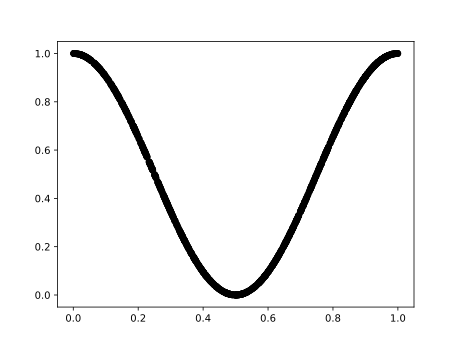
\includegraphics[width=\textwidth]{2som_courbe000_inputs.pdf}
			\caption{Cas d'entrées en deux dimensions~: $X\m{2}$ = $cos(X\m{1})$ \label{fig:cos}}
		\end{minipage}
		\begin{minipage}{0.33\textwidth}
			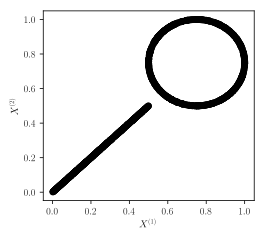
\includegraphics[width=\textwidth]{2som_mix_in.pdf}
			\caption{Exemple de dépendance en deux dimensions  \label{fig:mix}}
		\end{minipage}
	\end{minipage}
	\begin{minipage}{\textwidth}
		\begin{minipage}{0.33\textwidth}
			\includegraphics[width=\textwidth]{2som_inp_noU.pdf}
		\end{minipage}
		\begin{minipage}{0.33\textwidth}
			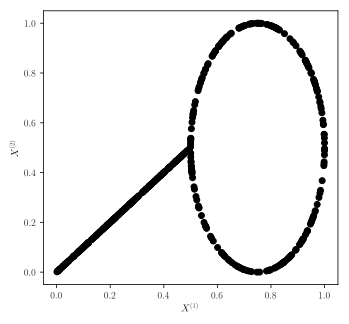
\includegraphics[width=\textwidth]{2som_mix001_in.pdf}
		\end{minipage}
		\begin{minipage}{0.33\textwidth}
			\includegraphics[width=\textwidth]{2som_square_in.pdf}
		\end{minipage}
	\end{minipage}
	
\end{figure}

\subsection{Matériel}

Les expériences présentées ici ont été réalisées en s'appuyant sur la librairie CxSOM \footnote{\url{https://github.com/HerveFrezza-Buet/cxsom}}, développée au sein de notre équipe.
Cette librairie C++ permet de créer des cartes de Kohonen simples ainsi que des architectures, régies par le modèle que nous avons présenté.
Une bibliothèque d'interface en python, pycxsom, est également disponible afin de faciliter les représentations des valeurs.
Les codes C++ et python que nous avons utilisé pour générer les expériences présentées dans ce chapitre est disponible sur git : REF.
Les connexions entre les cartes de l'architecture sont gérées par la librairie CxSOM, qui cherche à paralléliser au maximum les itérations de calcul. 
Typiquement, les itérations de tests sont performées en parallèle sur l'architecture de cartes.
Notons que la gestion du consensus passe par des mécanismes locaux aux cartes dans cette implémentation~: chaque carte envoie un signal aux cartes voisines lorsque son BMU n'est plus déplacée. Si une carte reçoit un signal de toutes ses connexions indiquant que leur BMU ne bouge plus et que son propre BMU n'est pas modifié, elle considère que le consensus est atteint.
Toutes les expériences présentées ici tournent sur un simple processeur i7.

\subsection{Méthodes}

Chaque jeu de donnée sert d'entrée d'apprentissage à une architecture de deux cartes 1D connectées réciproquement. Chaque carte a une taille fixée de 500 unités, indexées entre 0 et 1, et possède deux couches de poids $\w_e$ et $\w_c$. Les rayons de voisinage sont d'abord choisis à $r_e = 0.2$ et $r_c = 0.02$.
La génération des entrées suit le processus suivant~: $U$ est tiré uniformément dans $[0,1]$, puis les entrées $\inpx\m{1}$ et $\inpx\m{2}$ sont ensuite calculées à partir de la valeur de $U$.
L'apprentissage est réalisé sur un échantillon de 50000 itérations, générés aléatoirement. Les tests sont ensuite réalisés sur 5000 points générés aléatoirement selon la même distribution.



\section{Résultats}

Le premier but de cette étude est d'identifier des comportements \emph{systémiques} émergeant d'une architecture simple à deux et trois cartes, sur des entrées en deux et trois dimensions.
Nous avons identifié certains comportements au chapitre précédent, que nous évaluerons sur d'autres données entrées. Nous rappelons d'abord les comportements qu'on peut attendre d'une architecture de cartes.

\subsection{Entrées disposées sur un cercle : formulation d'hypothèses}

Revenons sur l'expérience présentée au chapitre \ref{chap:representation}, réalisée sur des entrées disposées selon un cercle. 

Analysons d'abord la forme des poids contextuels de $M\m{1}$, que nous avions tracés en figure~\ref{fig:w} sans les commenter. Les poids externes, en orange, présentent une disposition similaire à ceux observés dans la carte classique (b). Les poids contextuels, en bleu, présentent une forme de vagues, avec 7 valeurs de maximum allant de 0.5 à 1, et 6 minimum allant de 0.5 à 0.1. Ces maximum et minimum sont répartis en zones de taille équivalente sur la carte. 

Lorsqu'on s'intéresse aux tracés des échantillons, on remarque d'abord que les positions dans la carte $M\m{1}$ se répartissent en zones étant BMUs et zones mortes, dans lesquelles aucune entrée n'a gagné. C'est une première différence avec la carte indépendante, pour laquelle toutes les positions gagneront pour des entrées. Les zones dans lesquelles il y a des BMUs correspondent aux extremum des poids contextuels et leurs alentours. C'est un phénomène inhabituel pour une carte de Kohonen. Les entrées $\inpx\m{1}$, dans la carte classique (b), correspondent à la courbe de poids externe: la valeur du poids du gagnant est toujours très proche de la valeur de l'entrée. Dans la carte $M\m{1}$, les entrées externes $\inpx\m{1}$ orange sont proches de la courbe de poids externes, mais avec plus d'erreur de quantification.
Les deux points rouge et bleu ayant la même valeur de $x$ ont un BMU différent dans la carte $M\m{1}$, alors que ces deux échantillons ont le même BMU dans la carte apprenant indépendamment sur les valeurs de $x$. Ainsi, la carte connectée au sein de CxSOM différencie les échantillons en fonction de non seulement leur entrée externe, mais aussi de l'entrée de l'autre carte de l'architecture. La plage de valeurs des $\inpx\m{1}$ gagnant dans un des zones recoupe les plages de valeurs gagnant dans les zones situées à gauche et à droite. Par exemple, la zone dans laquelle l'échantillon rouge gagne, autour de $\bmu\m{1} = 0.25$. La partie des entrées située en dessous de la courbe de poids externe recoupe les valeurs d'entrées gagnant dans la zone précédente; la partie située au dessous de la courbe de poids externe recoupe des valeurs gagnant dans la partie suivante. Pour une entrée externe, le choix de la zone de BMU dans laquelle elle gagnera dépend alors de l'entrée contextuelle. 


Dans la carte $M\m{1}$, une unité se spécialise donc par rapport aux deux entrées et non pas une seule comme dans la carte indépendante: les entrées externes et l'entrée contextuelles. C'est bien ce à quoi on s'attendait en ayant deux couches de poids. Ce qui est intéressant est que cette différenciation est réalisée par la répartition des unités en un nombre fini de zones distinctes. Dans chaque zone, les unités sont BMUs pour un segment de valeurs d'entrée externe et contextuelles. Au sein d'une zone, la répartition des entrées externe selon le BMUs est ordonnée, comme ce serait le cas dans une carte auto-organisatrice classique. Le comportement de la carte au sein d'une zone reste donc similaire à celui d'une carte classique.

Deux zones adjacentes correspondent par ailleurs à des segments de valeur d'entrée en partie superposés, et des segments de valeurs d'entrées contextuelles différentes. Il s'agit d'une deuxième échelle d'organisation, qui garde également l'aspect ordonné d'une carte classique. Ces zones sont créées par auto-organisation~; aucun paramètre de la carte n'a été modifié pendant l'apprentissage pour former ces zones, et le nombre d'unités allouées par auto-organisation dans chaque zone est à peu près égal. La carte agit un peu comme une base de données structurée avec des indices primaires et des indices secondaires pour chaque neurone, l'indice primaire étant la zone de la carte, et l'indice secondaire la position dans cette zone.


Les résultats de cette expérience nous permettent donc de formuler les hypothèses suivantes concernant le comportement de cartes en une dimension~:

\begin{itemize}
	\item Les poids externes de chacune des cartes effectuent une quantification vectorielle correcte sur leurs entrées externe \ref{fig:qv}
	\item Les poids contextuels de chaque carte s'organisent en zones distinctes. Une zone correspond à un même intervalle de valeur pour $\inpx$ et $U$. Deux zones adjacentes encodent le même intervalle de valeurs pour $X$ mais des valeurs distinctes de $U$. \ref{fig:w} Ces zones se caractérisent par un étirement de la carte entre deux valeurs éloignées, apportant un aspect discontinu. Cette discontinuité passe en fait par la présence d'une zone peu dense de la carte contenant des n\oe{}uds qui ne seront jamais BMUs \ref{fig:w_zoom}. Nous verrons en section Prédiction que la formation de ces zones permet à la carte de prendre des décisions lors d'une phase de prédiction, ce qui n'est pas le cas autrement.
	\item La séparation des $U$ peut être vérifiée par une relation fonctionnelle entre $U$ et $\bmu$ dans chaque carte.
\end{itemize}

Nous chercherons à vérifier toutes ces observations sur d'autres dispositions d'entrées dans des structures de deux cartes, et nous nous demanderons si la création de zones dépend de la disposition des entrées~: une valeur de $X\m{1}$ correspondant à 1 (identité), 2 (cercle),3 , ou une infinité de valeurs de $X^{(2)}$ (carré $[0,1]^2$). Nous chercherons donc à savoir comment ces zones sont construites. Une caractéristique d'une carte de Kohonen est sa robustesse au bruit, une carte apprenant une représentation d'une structure d'entrées, même bruitée. 
Nous vérifierons si cette propriété se traduit également dans les architectures de cartes.

Nous étendrons ensuite notre étude aux structures de trois cartes apprenant sur trois entrées 1D connectées par un $U$ 1D. De cette manière, la connaissance de deux entrées et du modèle de relation nous permet de déduire la troisième entrée. Nous montrerons que cette tâche de prédiction est également effectuée par une architecture de trois cartes. Cette tâche de prédiction apparait comme une preuve expérimentale de l'apprentissage du modèle.
Nous pourrons enfin vérifier le comportement des cartes lorsqu'elles reçoivent plus d'une connexion contextuelle.

\begin{figure}
	\centering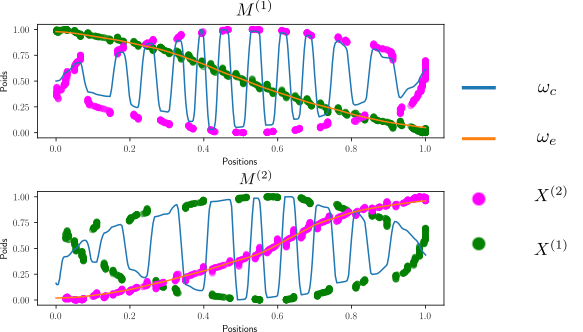
\includegraphics[width=0.9\textwidth]{2som_cercle_w.pdf}
	\caption{Représentation cartographique des poids et entrées lors d'une phase de test selon la position dans chacune des cartes. Nous remarquons que les poids d'une carte, par exemple la carte $M^{(1)}$ s'organisent en zones différenciant les valeurs de la paire $X^{(1)}, X^{(2)}$ et non seulement de la valeur de $X^{(1)}$. Deux zones adjacentes codent pour des valeurs de $X^{(1)}$ proches, mais $X^{(2)}$ différents. Au sein d'une même zone, les BMUs s'organisent sous la forme d'une mini carte sur les valeurs de l'entrée contextuelle. Ces zones se forment de manière auto-organisée. \label{fig:w}}
\end{figure}

\begin{figure}
	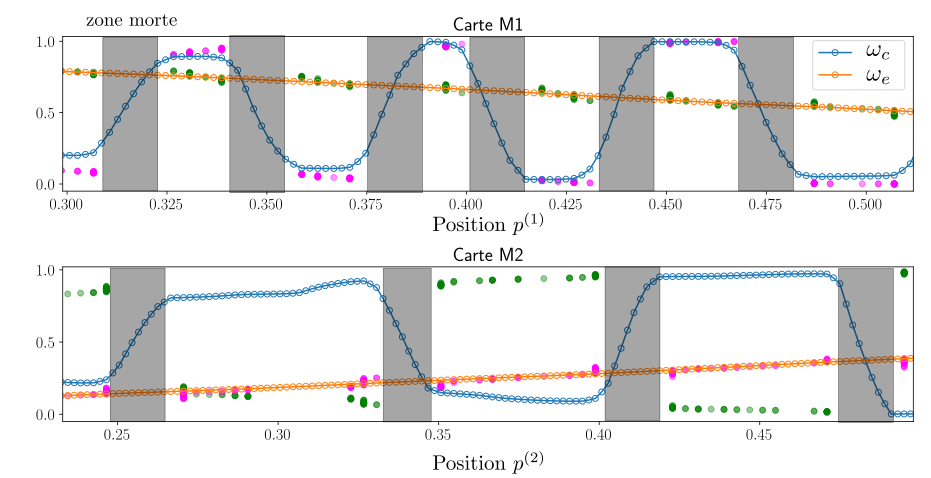
\includegraphics[width=\textwidth]{2som_cercle_w_zoom_with_nodes.pdf}
	\caption{Zoom sur la figure \ref{fig:w}. Nous y faisons apparaître la position sur la courbe des noeuds de la carte. Nous voyons que les zones grisées contiennent quelques n\oe{}uds qui ne sont jamais BMUsé; ce sont des zones mortes. Nous en concluons que la discontinuité introduite par la formation de zones est une "fausse" discontinuité et se produit en reliant des valeur de $\w_c$ éloignée en étirant une portion de carte morte. \label{fig:w_zoom}}
\end{figure}

\begin{figure}
	\includegraphics[width=\textwidth]{2som_cercle_err.pdf}
	\caption{Représentation de l'erreur de quantification sur les valeurs de $X^{(1)}$ et $X^{(2)}$. Le poids externe du BMU est proche de la valeur de l'entrée~; chaque carte possède donc une capacité de quantification vectorielle sur ses entrées. \label{fig:qv}}
\end{figure}

% \subsection{Quantification vectorielle sur les entrées externes}

% Une carte de Kohonen classique permet l'apprentissage de représentation sur ses entrées par quantification vectorielle. Elle extrait les structures sous-jacentes à la géométrie et topologie des points d'entrées sur un ensemble de vecteurs ordonnés.
% La qualité de la quantification sur chaque carte est une première condition à vérifier pour évaluer l'organisation d'une architecture.
% L'erreur de reconstruction d'une entrée par le poids de son BMU est d'abord un bon indicateur de la qualité de quantification vectorielle d'une carte~: toutes les entrées sont associées à un poids $\w\ext(\bmu)$ qui leur est proche.
% Nous attendons ainsi de chaque carte de l'architecture qu'elle ait une erreur de quantification faible sur l'entrée qu'elle a appris.

% \subsection{Différenciation de $U$ selon les BMUs: indicateur d'une mémoire associative}

% Nous appliquons une architecture de cartes à des tâches de mémoire associative sur des entrées multimodales.
% Le but de la mémoire associative est d'apprendre des données de plusieurs modalités et d'apprendre leurs associations. L'apprentissage des données indépendantes est donc un comportement nécessaire à cette mémoire associative. 
% Le but de la mémoire associative est d'apprendre des relations entre les entrées. Comme une carte cherche à extraire une structure dans les données de son espace d'entrée, observe t-on l'apprentissage d'une structure dans les relations entre entrées dans l'architecture de cartes ?
% Les expériences menées sur le cercle en 2D nous ont montré que les cartes s'auto-organisent de façon à ce que $U$ soit une fonction du BMU $\bmu$ dans chaque carte. Nous vérifierons cette propriété sur les nouveaux jeux d'entrées.

% \subsection{Découpage d'une carte en zones grâce aux poids contextuels}

% Enfin, nous remarquerons que cet apprentissage de relations passe par la disposition en zones auto-organisées au sein d'une carte. Ces zones, nous l'avons vu, déterminent la BMU de chaque carte en fonction de l'ensemble des entrées et non seulement de l'entrée de la carte en question. Ces zones ne marquent pas l'apprentissage d'une relation: dans les cas ou les entrées sont indépendantes, la carte se divise quand même en zones distinctes. La présence de zones est spécifique au comportement de l'architecture CxSOM.

\subsection{Vérification des hypothèses sur les autres jeux de données d'entrées}

Nous tracons maintenant le 

\begin{figure}
\begin{minipage}{0.66\textwidth}
	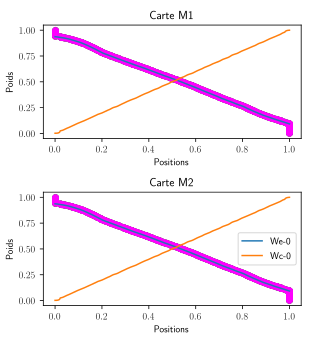
\includegraphics[width=\textwidth]{2som_id_w.pdf}
	\caption{Représentation cartographique des poids et entrées pour la disposition identité}
\end{minipage}
\begin{minipage}{0.33\textwidth}
	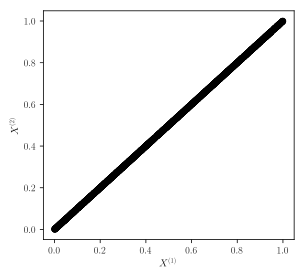
\includegraphics[width=\textwidth]{2som_id_in}
\end{minipage}
\end{figure}

\begin{figure}
	\begin{minipage}{0.66\textwidth}
	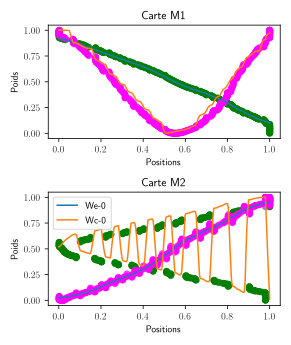
\includegraphics[width=\textwidth]{2som_cos_w.pdf}
	\caption{Représentation cartographique des poids et entrées pour la disposition cos}
	\end{minipage}
	\begin{minipage}{0.33\textwidth}
		\includegraphics[width=\textwidth]{2som_cos_in.png}
	\end{minipage}
\end{figure}

\begin{figure}
	\begin{minipage}{0.66\textwidth}
		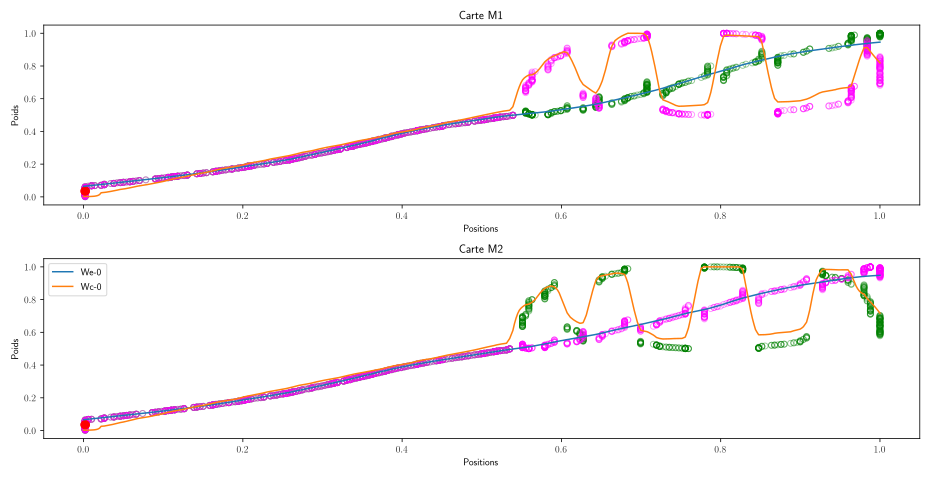
\includegraphics[width=\textwidth]{2som_mix_w.pdf}
	\caption{Représentation cartographique des poids et entrées pour la disposition mix}
	\end{minipage}
	\begin{minipage}{0.33\textwidth}
		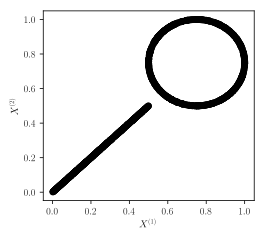
\includegraphics[width=\textwidth]{2som_mix_in.pdf}
	\end{minipage}
\end{figure}

\begin{figure}
	\begin{minipage}{0.66\textwidth}
		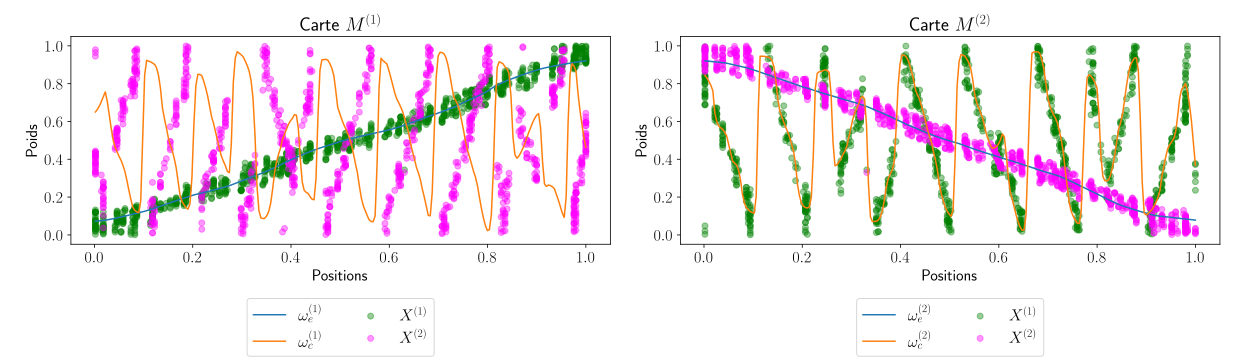
\includegraphics[width=\textwidth]{2som_square_w.pdf}
	\caption{Représentation cartographique des poids et entrées pour la disposition mix}
	\end{minipage}
	\begin{minipage}{0.33\textwidth}
		\includegraphics[width=\textwidth]{2som_square_in.pdf}
	\end{minipage}
\end{figure}


\begin{itemize}
	\item Organisation en zones dès que besoin de découpler deux valeurs de U
	\item Le comportement traduit l'existence de plusieurs valeurs de U pour une même entrée, sans forcément qu'une relation existe. Dans tous les cas, la carte effectue un découpage selon U.
	\item Lorsque relation il y a, ce découpage permet de faire de la prédiction.
\end{itemize}

\subsection{Discussion}

Indices primaires et secondaires observés en biologie \cite{ballard_cortical_1986}, avec accent sur le fait que ce n'est pas exactement pareil. 
Motifs auto-organisés de découpage en zones

Introduction de discontinuités dans une carte de Kohonen, mais en contrepartie présence de nombreux noeuds morts.
On observe que + on a de valeurs possible pour Y pour un meme X, moins on aura de noeuds morts dans les zones de discontinuité. 
Par ailleurs, organisation de la carte au sein d'une zone pour eviter les noeuds morts.

Ces architectures de quelques cartes sont des architectures \emph{élémentaires}: toute architecture comportant plus de cartes pourra être construite à partir de petits modules. Nous considérerons les comportements observés dans ce chapitre comme des comportements élémentaires des architectures de cartes.


%tracé pour les valeurs sur le cercl

\section{Prédiction d'entrée}

L'observation des comportements des cartes sur des entrées géométrique nous a fourni quelques éléments d'analyse des mécanismes d'organisation y occurrant. 
Nous avons également pu définir des outils de mesure de l'organisation des cartes.
Nous avons vu que le modèle, défini par la variable cachée, était appris dans chacune des cartes de l'architecture grâce aux connexions entre cartes.
Nous utilisons maintenant cet apprentissage du modèle dans une tâche de prédiction d'entrée.

Cette utilisation en tant que prédiction a d'abord une valeur applicative, car il s'agit d'un cas d'utilisation possible de l'apprentissage du modèle par une carte. Par ailleurs, la prédiction permet également de valider l'apprentissage du modèle par l'architecture. Par exemple, dans le cas de données réelles, le modèle d'entrée n'est pas forcément connu. La prédiction permet alors de valider l'apprentissage du modèle.

Rappelons la structure utilisée pour la prédiction (voir figure~\ref{fig:schema_pred})~: après apprentissage, nous choisissons une des cartes comme carte prédictive. Lors de la phase de prédiction, cette carte ne reçoit plus d'entrée externe, mais seulement les entrées contextuelles venant des autres cartes de l'architecture. 
Les autres cartes reçoivent quant à elles toujours leurs entrées externes et contextuelles. La phase de prédiction est une phase de test durant laquelle les poids de toutes les cartes ne sont pas mis à jour. Les règles de calcul et paramètres sont conservés entre apprentissage et prédiction. La carte ne recevant pas d'entrée externe prend simplement comme activité globale son activité contextuelle.

\begin{figure}
	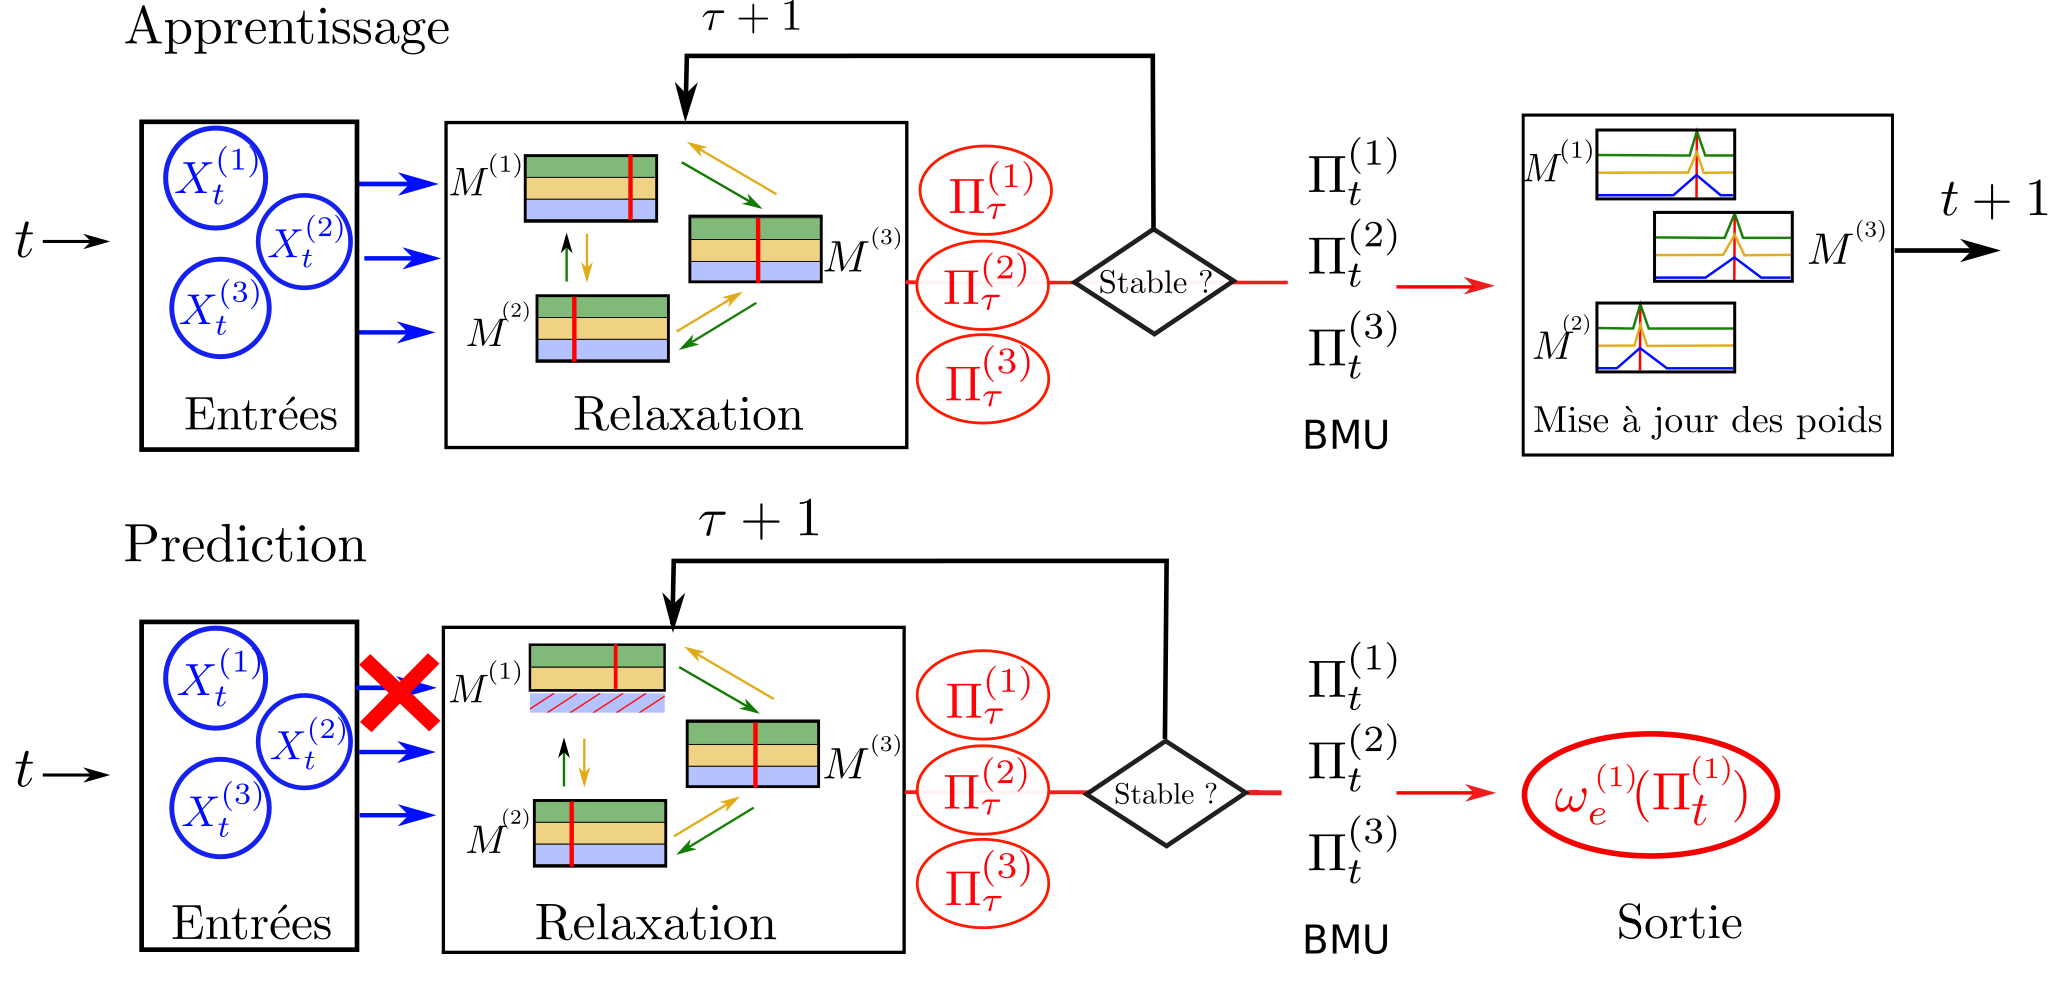
\includegraphics[width=\textwidth]{learning_tests.pdf}
	\caption{Schéma descriptif des opérations effectuées lors de l'apprentissage et de la phase de prédiction.\label{fig:schema_pred}}
\end{figure}


\subsection{Entrées géométriques}

Nous testons d'abord la prédiction sur des dispositions d'entrées géométriques.
Les tâches de prédiction seront possible dans le cas où la connaissance des entrées et du modèle détermine la troisième valeur d'entrée. Dans le cas du cercle en deux dimensions, la prédiction n'est ainsi pas possible.
Nous prendrons comme premier exemple des entrées disposées sur un cercle en deux dimensions plongé et pivoté dans l'espace en 3D \ref{fig:cercle3}. De cette manière, la connaissance de deux des trois coordonnées permet de déterminer la troisième avec précision.
Nous utilisons pour cela une architecture de trois cartes 1D, toutes connectées entre elles.  
En deuxième exemple, nous présentons les résultats sur une architecture de trois cartes 2D, apprenant sur une surface, une sphère, plongée et pivotée dans un espace en six dimensions. Encore une fois, la connaissance de deux entrées sur trois ainsi que du modèle nous permet de prédire la dernière coordonnée, et nous souhaitons vérifier ici si la présentation de deux entrées sur trois à l'architecture permet de prédire la troisième.

La figure \ref{fig:w_cercle} présente la disposition des poids des trois cartes de l'architecture ainsi que des entrées associées. Comme dans la version à deux cartes, les poids contextuels s'organisent en plusieurs zones au sein desquelles la valeur de $U$ est située dans une même plage de valeur. La figure \ref{fig:pred_cercle} présente l'erreur obtenue lors de la phase de prédiction. L'entrée $X\m{1}$ n'est alors pas présentée à la carte et sa valeur est prédite par $\w\ext\m{1}{\bmu\m{1}}$. Nous voyons ici que la prédiction est bien réalisée. Remarquons que la disposition en lignes horizontales n'est pas anodines: elle correspond aux zones définies par les valeurs des poids contextuels d'une carte.

\begin{figure}
	\centering\includegraphics[width=0.9\textwidth]{3som_cercle_w.pdf}
	\caption{\label{fig:w_cercle}}
\end{figure}

% \begin{figure}
% 	\centering\includegraphics[width=0.9\textwidth]{pred_anneau005_inputs.pdf}
% 	\caption{\label{fig:pred_anneau}}
% \end{figure}


\begin{figure}
	\includegraphics[width=0.9\textwidth]{prediction_x2.pdf}
	\caption{\label{fig:pred_cercle}}
\end{figure}





\subsection{Entrées réelles~: application sur un drône}

Nous sortons du cadre des entrées simulées pour nous placer dans un cas de contrôle réel. Nous disposons d'un drône quadricoptère, commandé à distance. Ce drône possède une caméra frontale ainsi qu'un ensemble de capteurs internes. Chacun de ces capteurs peut être considéré comme une modalité d'un espace multimodal. A ces modalités s'ajoute la modalité correspondant à la commande envoyée au drône.
Le principe est d'apprendre, à l'aide d'une architecture de cartes, les relations existants entre les modalités des capteurs et de la commande afin d'ensuite prédire la commande à envoyer à partir des capteurs.
Afin que les relations entre la commande et les capteurs soient significatives, nous nous placons dans un cas d'application particulier: le drône vole dans un couloir étroit, en ligne droite. Le but du drône est alors de voler en avant dans le couloir, sans toucher les murs.
Le but de cette expérience est de démontrer la tâche de prédiction en situation réelle. Nous évaluerons ainsi la robustesse de l'algorithme à des données bruitées, et la capacité de CxSOM à réagir en temps réel malgré la relaxation.

\subsubsection{Méthode expérimentale}

Le drône utilisé pour l'expérience est un quadricoptère. Il possède une caméra frontale.
Le drône est contrôlé à distance par un ordinateur; la commande est réalisée en envoyant l'accélération angulaire du drône autour de ses trois axes de rotation.
Nous avons accès aux données des capteurs internes, notamment la vitesse linéaire courante selon chaque axe de déplacement.

le drône se déplace dans un couloir étroit.
Dans le cadre de l'expérience, nous extrayons deux éléments visuels spécifiques au couloir à partir de la caméra du drône: l'abscisse du point de fuite du couloir $x$. Nous calculons également la différence entre les angles du couloir, notée $\varphi$. Ces valeurs sont illustrées en figure~\ref{fig:drone}.
Le drône se déplace dans un couloir, à hauteur constante et vitesse constante.
La commande générant le déplacement en avant du drône (tangage) est maintenue constante. Les commandes permettant le déplacement en largeur sont alors $\omega$ et $\rho$. Dans le cadre de cette expérience, nous contrôlerons uniquement $\rho$.
Enfin, la vitesse linéaire en largeur du drône peut être récupérée à chaque instant; nous la notons $v$.
Nous avons ainsi quatres modalités lors du déplacement du drône: $x$, $\varphi$, $\rho$ et $v$.
Nous construisons une architecture CxSOM sur ces quatres modalités, composée de quatre cartes connectées chacune aux trois autres.
Une phase d'apprentissage est réalisée sur des déplacements du drône contrôlés humainement. Notons que lors de cette phase, nous avons utilisé un système de contrôle PID pour assister la commande humaine. Cette phase d'apprentissage est réalisée hors ligne pour que les données soient réparties aléatoirement.
Après apprentissage, nous effectuons une phase de prédiction. Lors de cette étape, la commande $\rho$ n'est plus présentée à la carte correspondante. Nous envoyons alors le poids externe du BMU de cette carte comme commande du drône. Cette étape est réalisée en ligne, sur des trajectoires réelles du drône.

La figure \ref{fig:drone_inp} présente la répartition des entrées présentées au drône. Nous avons tracé les dépendances entre chaque modalité. Nous remarquons sur la figure qu'une dépendance forte se dégage entre les entrées ?? et ??, ainsi que ?? et ??. Si les cartes apprennent correctement le modèle liant les entrées, la prédiction peut être réalisée.
Ces dépendances sont très bruitées. Cette expérience en conditions réelles nous permettra d'observer la résistance au bruit de la prédiction.

%TODO mettre disposition des entrées.

\subsubsection{Résultats}
La carte associée à $\rho$ possède donc une couche de poids externe et trois couches de poids contextuels. Ces poids sont représentés en figure \ref{fig:drone_w}. L'organisation des poids contextuels rappelle celle observé dans des conditions géométriques: les poids contextuels définissent des zones. Contrairement à l'expérience réalisée sur un cercle, la taille de ces zones dépend de la couche de poids contextuel définie. 

\begin{figure}
\begin{minipage}{0.5\textwidth}
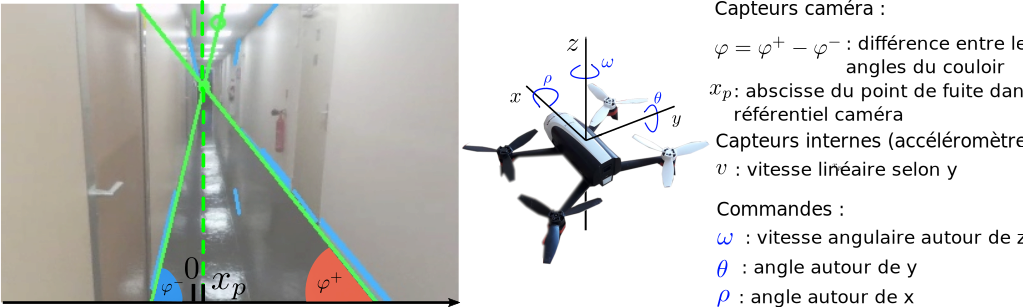
\includegraphics[width=\textwidth]{visudrone}
\end{minipage}
\begin{minipage}{0.5\textwidth}
\includegraphics[width=\textwidth]{dronesteup}
\end{minipage}
\caption{Disposition des capteurs utilisés pour l'experience}
\label{fig:drone}
\end{figure}

\begin{figure}
\includegraphics[width=\textwidth]{dronemap}
\caption{Disposition des poids de la carte $\rho$ après apprentissage et exemple de calcul d'activité}
\label{fig:drone_w}
\end{figure}

\subsubsection{Discussion}
Ici on ne cherchait pas à comparer avec des valeurs théorique, mais on observe que le drone ne tape pas les murs
Illustration de la capacité de prédiction et mémoire associative
Resistance au bruit

Calcul des dépendance entre les entrées et la commande:
PCA sur les entrées, calcul de MI après apprentissage

\section{Conclusion}


\ifSubfilesClassLoaded{
    \printbibliography
    %\externaldocument{../main.tex}   
}{}
\end{document}